\documentclass[twocolumn]{revtex4-2}

\usepackage{bm}
\usepackage{hyperref}
\usepackage{graphicx}
\usepackage{subcaption}
\usepackage{tikz}
\usetikzlibrary{arrows,shapes,automata,backgrounds,petri}
\usepackage{natbib}

\begin{document}
\raggedbottom
\title{Electrolysis of Water}
\author{Sixten Nordegren}
\affiliation{Stockholm University: Fysikum}

\date{\today}

\maketitle
\section{Introduction}
Water electrolysis is the process of separating the molecules of water $H_2O$ Into it's 
constituents $H_2$ and $O_2$ gas. This is done in two separate chemical reactions. The
oxidisation of water,

\begin{equation}
	2H_2O \rightarrow O_2 + 4 H^+ +4e^- 
	\label{eq: oxidisation}
\end{equation}
and the reduction of Hydrogen ions.
\begin{equation}
	2 H^+ + 2e^- \rightarrow H_2
	\label{eq: reduction}
\end{equation}

The reaction described above does not happen all by itself. An electrical field needs to be
applied over the water for the oxidisation to be possible. The 
thermo-dynamical minimum ($\text{E}_{\text{min}}$) voltage that needs to be applied is $1.23$ V. 

\par
Water electrolysis by itself is a fairly slow process. Excess energy is used in order to increase
the rate of the reaction as well as to overcome small hindrances in the liquid, the excess energy 
is called \textbf{Overpotential}. Beyond that, electrolyte
in the combination with catalysts are other ways to optimize the process. 
\par
The usage of water electrolysis as a tool for hydrogen production has a lot of upsides. Water being the 
only ingredient and the single byproduct being oxygen makes the process comparably
environmentally friendly to it's alternatives \cite{DOSSANTOS2017563}.
\par 
As of today water electrolysis is responsible for about $4\%$\cite{ZENG2010307} of the global Hydrogen
production. The reason for the quite low market share in spite of all the previously mentioned upsides 
is that the process is simply to inefficient and it's materials to expensive\cite{SHIVAKUMAR2019442}.

To find new materials that could make the process more effective is currently an active field of 
research.

The aim of the experiment is to find what catalysts correlate to the most effective form of 
hydrogen and oxygen production.

\par 
The Tafel equation describes the overpotential as a function of the rate of the electrochemical reaction.\cite{bard2001electrochemical}

\begin{equation}
	\eta = \pm A \times \log_{10}{\left(\frac{i}{i_o}\right)}
	\label{eq: tafel}
\end{equation}


\begin{figure}[b]
	\centering
	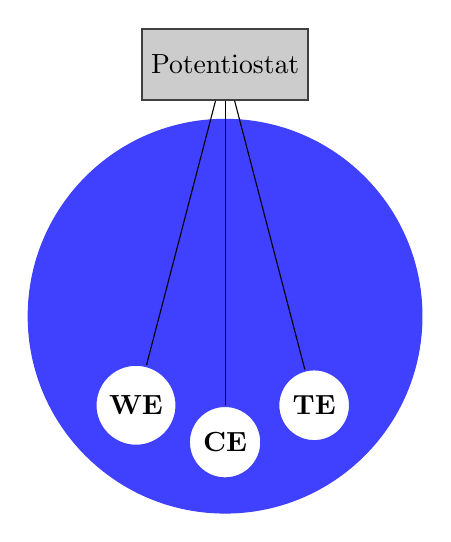
\begin{tikzpicture}[node distance = 1.6cm]
	  \tikzstyle{electrode}=[circle,thick,draw=blue!75,fill=white!20,minimum size=6mm]
	  \tikzstyle{container}=[place,draw=blue!75,fill=blue!75, minimum size= 50mm]
	  \tikzstyle{potentiostat}=[rectangle,thick,draw=black!75,
				  fill=black!20,minimum size=9mm ]
	
	\node (center_top) {};
	\node (center_top+)[potentiostat] [above of= center_top]{Potentiostat};
	\node (center_center) [container] [below of= center_top]{};
	\node (center_bottom)[electrode] [below of= center_center] {\textbf{CE}};
	\node (right_bottom)[electrode] [below right of= center_center]{\textbf{TE}};
	\node (left_bottom)[electrode] [below left of= center_center]{\textbf{WE}};

	\draw (center_top+) -- (left_bottom) ;
	\draw (center_top+) -- (right_bottom) ;
	\draw (center_top+) -- (center_bottom) ;


		%\draw (a2) -- (a2.1);
		%\draw (a2) -- (b1);
		%\draw (a2) -- (b3);
		%\draw (a2) -- (c1);
	\end{tikzpicture}
	\caption[]{Diagram of experimental setup.\newline
	\textbf{CE}: Counter electrode \newline
	\textbf{WE}: Working electrode \newline
	\textbf{TE}: Test electrode \hspace{1.9cm}
\label{fig: potentiostat}}

\end{figure}
\section{Method}
\subsection{Catalyst testing}
Three electrodes are lowered down into water with the electrolyte mixed in with it.
One Working Electrode (\textbf{WE}) from which all the measurements are made. One counter
electrode (\textbf{CE}) that close the circuit and together with the \textbf{WE} establishes a 
homogeneous electric field. Lastly a final measuring electrode (ME) is inserted
into the mixture in order to make reliable measurements of the working electrode. See \ref{fig: potentiostat}
for a diagram of the setup.

\begin{figure}[t]
	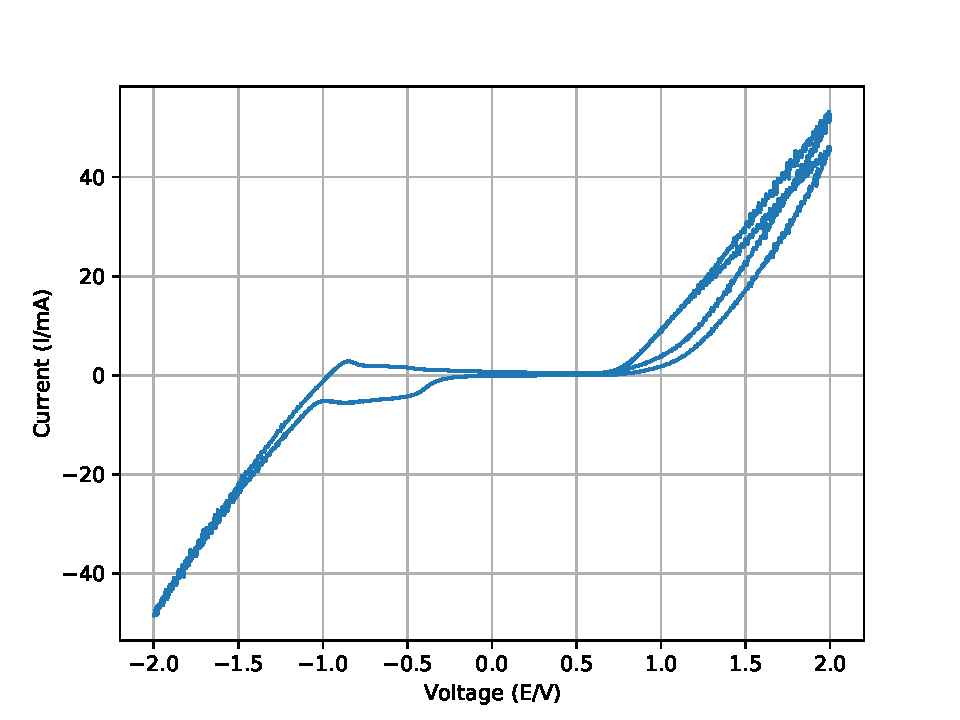
\includegraphics[width=0.9\linewidth]{/home/sixten/water_electrolysis/data_analysis/plots/data_plot_1.pdf}
	
	\caption{Plot from the first Platinum Platinum measurement \label{fig:I_Plt_1}}
\end{figure}



On the end of the \textbf{WE} and the \textbf{CE} two metals are attached acting 
as catalysts for the chemical reaction. 

\par
Potential builds up potentiostat via the \textbf{WE} and later the \textbf{CE}. This potential cycles
between $\pm 2$ V in order to determine when if at all, current starts flowing through the circuit.
This data is saved and processed inside a computer connected to the potentiostat.

See \ref{fig:I_Plt_1} for an example of what data the procedure described above might produce.

\subsection{Gas collection}
Empty tubes are lowered down into the water resting above the catalyst and subsequently
have their air sucked out of them. Allowing the bubbles that inevitably form on the
catalyst to float up into the empty tubes. 

\par 
All of the gas doesn't make it into the tubes but the amount that does are about equal
for either reaction so the gases that gets trapped inside of the tubes is representative
of the actual gas produced, proportionally to one another.

\par 
When placing down the tubes and sucking out all the air there is a need to get into 
physical contact with the electrolyte. Since $0.1$ Mol KOH is highly corrosive we change 
it out for standard $1.0$ Mol HCL (salt) which is safer.
\par 
The potentiostat is replaced with a more classical potential generator. Running a much
stronger current through the circuit.
\par


\subsection{Analytical methods}
The potentiostat goes through a set number of cycles for each measurement.
This is done in order to make minimize any random errors that might occur. Unfortunately
each cycle wasn't exactly the same length as the previous one, for reasons probably only
known to the makers of the potentiostat, so in order to take sensible averages
some points from the longer data cycles where cropped.
\par
The removed sections of data comes from the middle of the data sets. Points that, wont be
used for further analysis anyway.
\par
In order to standardize the measurements we need to control for the differing sizes of the catalysts
that where in the water. Therefore we divide each data point by the area of the corresponding
catalyst in order to attain the current density.
\par
We expect the relationship of the current density and the overpotential to be of exponential
characteristic so we plot the $\bm{\log{()}} $ of a part of the data that represents the overpotential.
To plot the data for both the Oxygen evolution reaction (\textbf{OER}) and the hydrogen evolution
reaction \textbf{HER} we need to analyze different parts separately due to the nature of the logarithm
as a function. See \ref{figure: CD_plat} for a graphical representation of this process.

\par
We then use the Tafel equation to approximate a value for the Tafel slope ($A$). And then compare
the theoretical value to the experimental one as a function of exchange current density.

\section{Results}
All the data for all the experiments can be found at \url{https://github.com/SixtenNordegren/Water_Electrolysis
} along with the code 
for of the data analysis. Due to the magnitude of data collected I won't be able to
give each and every data set collected a fair showing. I will be presenting a selected 
few sets of data.


\begin{table}[h]
\begin{tabular}{|c|c|c|c|c|}
	\hline
	& Copper & Platinum & Nickel & Gold \\
	\hline
	Width $(\text{cm})$&$0.65\pm 0.1$ &$0.80 \pm 0.1$&$0.65 \pm 0.1$&$0.65 \pm 0.1$\\
	\hline
	Length $(\text{cm})$ &$0.60 \pm 0.1$&$1.50 \pm 0.1$&$1.30 \pm 0.1$&$1.60 \pm 0.1$\\
	\hline
	Area $(\text{cm}^2)$ &$0.7 \pm 0.2$&$1.2 \pm 0.2$&$1.4 \pm 0.2$&$0.9 \pm 0.1$\\
	\hline
\end{tabular}
	\caption{Table of measured length of catalyst submerged into water.\label{table: area}}
\end{table}

\begin{figure}[h]
	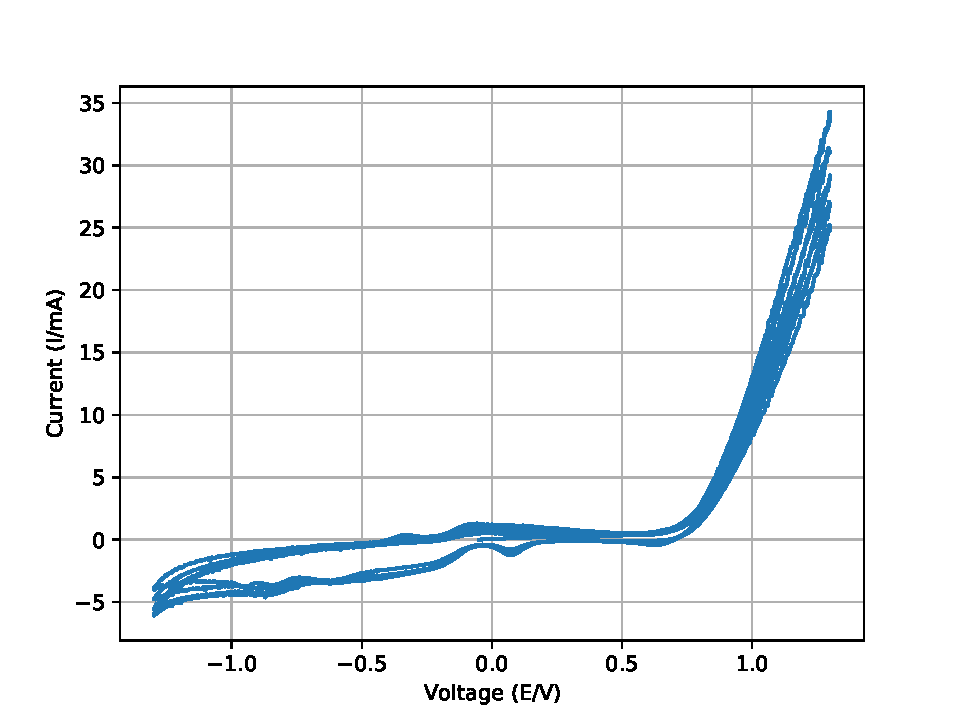
\includegraphics[width=0.95\linewidth]{~/water_electrolysis/data_analysis/plots/data_plot_9.pdf}
	
	\caption{Water electrolysis with gold as the \textbf{WE}, doing a particularly poor job (Pt 
	is \textbf{CE})\label{figure: Au_Pt_current}}
\end{figure}

In table \ref{table: area} we can see the measurements of what part of the metal catalysts
that ended up in the water. This was done by extracting the catalyst after the experiment
was performed and measuring the wet parts of the catalyst with a ruler. Since the catalysts 
where hanging from cables into the water, they couldn't be held perfectly perpendicular to 
the water surface, which often resulted in a slanted mark of water on the electrode.
In those cases we simply averaged the length of the wet sides and calculated the area as 
if they were a perfect rectangles. 


\begin{figure*}[t]
	\centering
	\begin{minipage}{0.45\linewidth}
	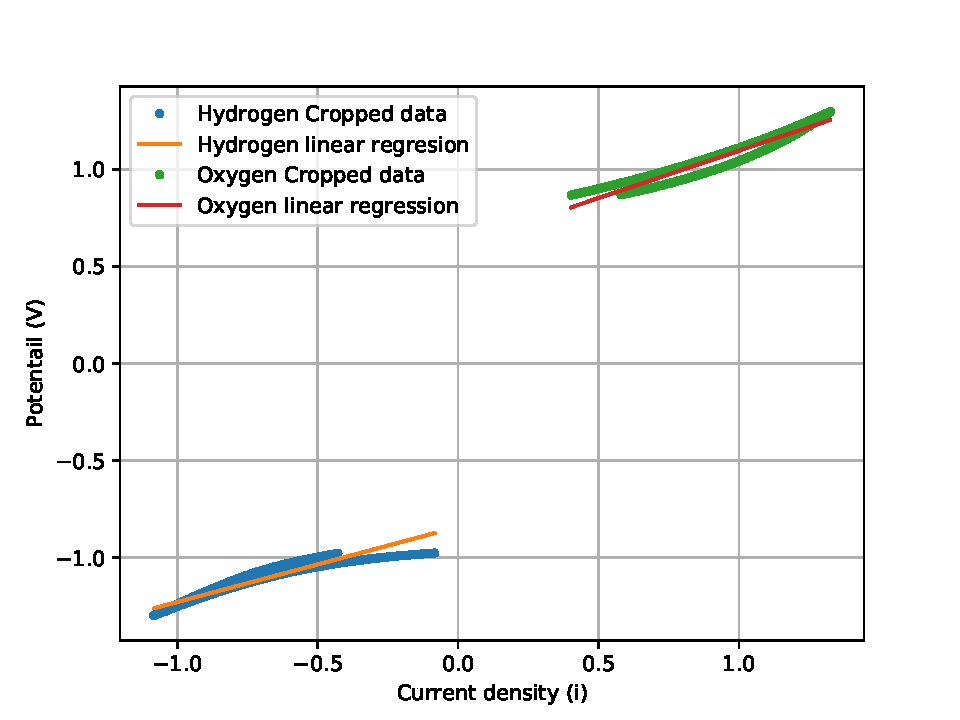
\includegraphics[width=0.9\linewidth]{/home/sixten/water_electrolysis/data_analysis/plots/Cropped_data.pdf}
	\caption{Logarithm of the current exchange density. With linear regression for both 
	the oxidisation and the reduction.\label{figure: CD_plat}}
	\end{minipage}
	\begin{minipage}{0.45\linewidth}
	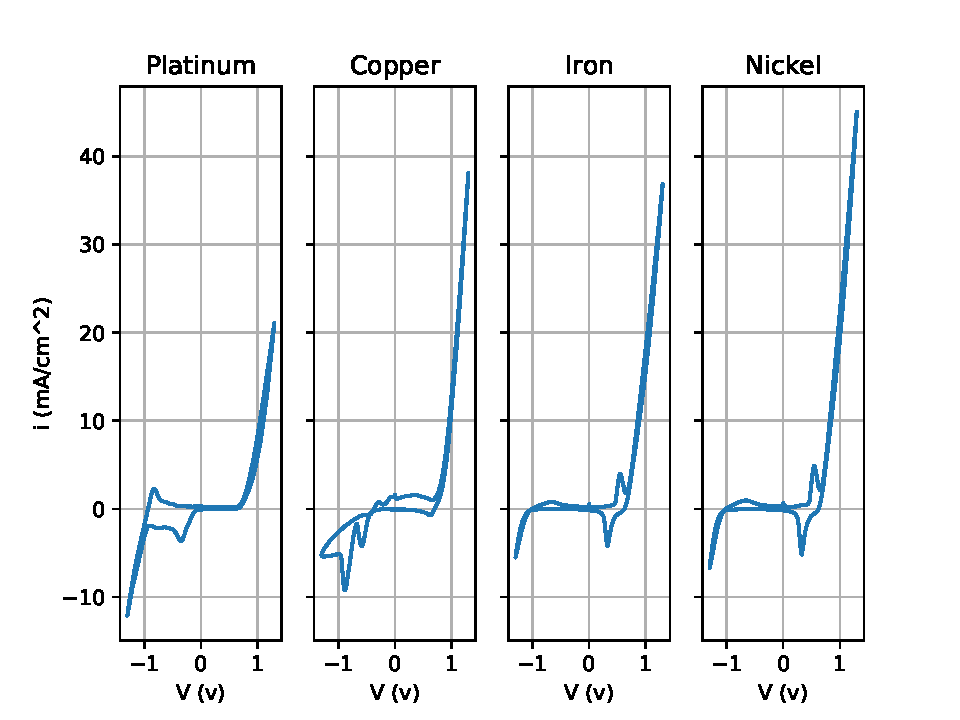
\includegraphics[width=0.9\linewidth]{/home/sixten/water_electrolysis/data_analysis/plots/multiplot_avg_li.pdf}
	\caption{Multiple data plots with average cycles. \label{figure: Average cycle}}
	\end{minipage}
\end{figure*}
In table \ref{table: ecd_H} and \ref{table: ecd_O} we see the exchange current densities.
These values where extracted by performing a linear regression on 
different parts of the logarithm of measured data and then solved for when $\eta = 0$. This is a good method a good chunk of the 
time, but some samples are bad enough catalyst as to barley 
have a reaction happen at all an example of this can be seen in figure \ref{figure: Au_Pt_current}.
This in turn leads to some very inaccurate exchange current densities. So if 
a very perceptive reader find some of the values odd, compared to other literature values. That would
be why.

\begin{table}[h]
\begin{tabular}{c | c}
Material & $i_{ecd}$ $(A/cm^2)$ \\
\hline
\hline
Platinum & $2.92 \pm 0.04$\\ 

Copper & $4.7 \pm 0.5$\\ 

Gold & $0.032 \pm 0.003$\\ 

Nickel & $10.2 \pm 0.1$\\ 

Iron & $1.343 \pm 0.007$\\ 

\end{tabular}
	\caption{Table of current exchange current density for the hydrogen reaction\label{table: ecd_H}}
\end{table}

\begin{table}[h]
	\begin{tabular}{c|c}
		Material & $i_{ecd}$ $(A/cm^2)$ \\
		\hline
		\hline
		Platinum & $0.32 \pm 0.01$\\ 

		Copper & $0.19 \pm 0.01$\\ 

		Gold & $0.64 \pm 0.01$\\ 

		Nickel & $0.57 \pm 0.01$\\ 

		Iron & $0.005 \pm 0.007$\\ 

	\end{tabular}
	\caption{Oxygen Exchange current densities\label{table: ecd_O}}
\end{table}

\begin{table}[h]
	\begin{tabular}{c | c}
		HER & V $H_2$ (mL) \\
		\hline
		\hline
		Pt &$ 2 \pm 0.5$ \\
		Au & $2.6 \pm 0.5$ \\
	\end{tabular}
	\caption{Collected Hydrogen gas\label{table: gases}}
\end{table}
\par
The gas that was collected can be found in in table \ref{table: gases}. Originally we were supposed to 
measure the oxygen production as well as the hydrogen production, but after  the change of electrolyte
the amount of $O_2$ gas produced was to small to measure.

In figure \ref{fig: tafel} we see the Tafel equation compared to some of the collected data.
\footnote{The data for the current exchange density is inverted for the Tafel equation} The
Tafel equation is calculated with the Tafel slope.

\begin{equation}
	 A = \mp\frac{\eta}{\log{(i/i_o)}} 
\end{equation}


\begin{equation}
	A \approx 1.76 \pm 0.01 V
	\label{eq: tafel_slope}
\end{equation}
Which is in turn generated by solving the Tafel equation \ref{eq: tafel} repeatedly for each
data point in the current exchange density, and taking the average.

We can see the overpotential predicted by the Tafel equation in \ref{fig: tafel} compared
to the collected data. The figure is in quite good agreement for the largest values, but diverges
quite quickly for the smaller ones, this is due to the logarithmic nature of the Tafel equation\ref{eq: tafel}.


\section{Discussion} 

The question, what catalyst is best fitted to make either reaction as efficient as 
possible among those we tested is a rather intuitive experiment by itself. But what 
would make a catalyst effective? Since we are trying to create hydrogen we would want a 
catalyst that promotes lot's of \textbf{HER} reactions \ref{eq: reduction} to take place. Current
in this case makes for a good variable to keep track of that will measure this. 
\par 
The production of hydrogen moves electrons that is freed at the anode and recombine
at the cathode. Closing the circuit and providing current. The more current is in the 
circuit, the more reactions are taking place the higher the current
\footnote{At least in principle, as we shall see later on in the discussion this isn't 
the whole story.}
.


The 
graphs from the initial data is already a pretty good indicator weather the catalyst
was an effective one or not. See the stark contrast between figure \ref{fig:I_Plt_1} and 
\ref{figure: Au_Pt_current}. We can already tell that when gold has a large negative 
potential over it, the total current is very low. At least when compared to the Platinum.
In other words when Gold have a large negative charge acting as a catalyst for \textbf{HER}
very few electrons seems to make it to the cathode and create hydrogen gas. Making it a 
bad catalyst. 
\par
To distinguish among the more effective catalysts however,
we need to look a little closer. Since we risk letting the different sizes 
of the catalyst dictate the current.
\par 
The need for more detail seems to be unnecessary when it comes to the hydrogen production
electrode, since \textbf{Pt} (Platinum) seems to outmatch all the other alternatives by mile.
It's the only catalyst among those that we tested that at all managed to dip below a current
density of $ - 10\text{mA/cm} ^2$ and outclassed all the other alternatives. For oxygen production 
however there where plenty of viable alternatives, however it would seem that (\textbf{Ni}) Nickel would 
come out on top, reaching all the way up to the high $40(\textbf{mA}/\textbf{cm}^2)$'s. See figure
\ref{figure: Average cycle} for a comparison between some of the current density measurements.

\subsection{Error sources}
The largest source of error for this experiment, or rather it's largest failure. Was 
the inability to measure the oxygen produced by the \textbf{OER}. This is strange 
since we did manage to measure a quite large current for plenty of different catalyst.
\par
Moreover It seems that the gold managed to outproduce platinum in the \textbf{HER}.
\begin{enumerate}
	\item New electrolyte \\
		When measuring the gas intake we used a new electrolyte $1$ Mol HCl instead of the
		0.1 Mol KCl used in previous experiment. This seemed to have to a decrease in water oxidisation
		and an increase in oxidisation of whatever catalyst was used at the time. The precise
		reason for this is hard to place exactly. One reason might be that the PH value is 
		different for each of the electrolytes PH 1Mol HCl mixture is around 7 and the 0.1Mol KCl
		is about 13. This might change the overpotential for either reaction slightly but due 
		to the higher potential overall used in the experiment this seems minor.
	\item Mixture of different elements \\
		During the process different catalysts where tested sometimes in the same 
		water-electrolyte bath. This might have had an adverse effect for either of 
		the reactions. Particularly the gold reaction outproducing the platinum might
		be due to platinum ions floating around in that same experiment.
	\item Irregular tube placement\\
		It is also possible that, the capturing tubes. In-between measurements where moved
		between the hydrogen capture experiment and the gold capture measurement. Leading 
		a hight yield in gas from the gold.
\end{enumerate}

The determination of effective catalysts where thankfully more reliable. However even this experiment
isn't perfect. 
For most of the measurements there were a slight bump at the beginning of the \textbf{HER} this is due to
Oxygen that's left on the catalyst from when it had a different charge which can react after the polarity
switch and causing some current not pertaining to the experiment. To counteract this we pumped in some 
nitrogen but still didn't manage to entirely curb the occurrence.

\begin{figure}[h]
	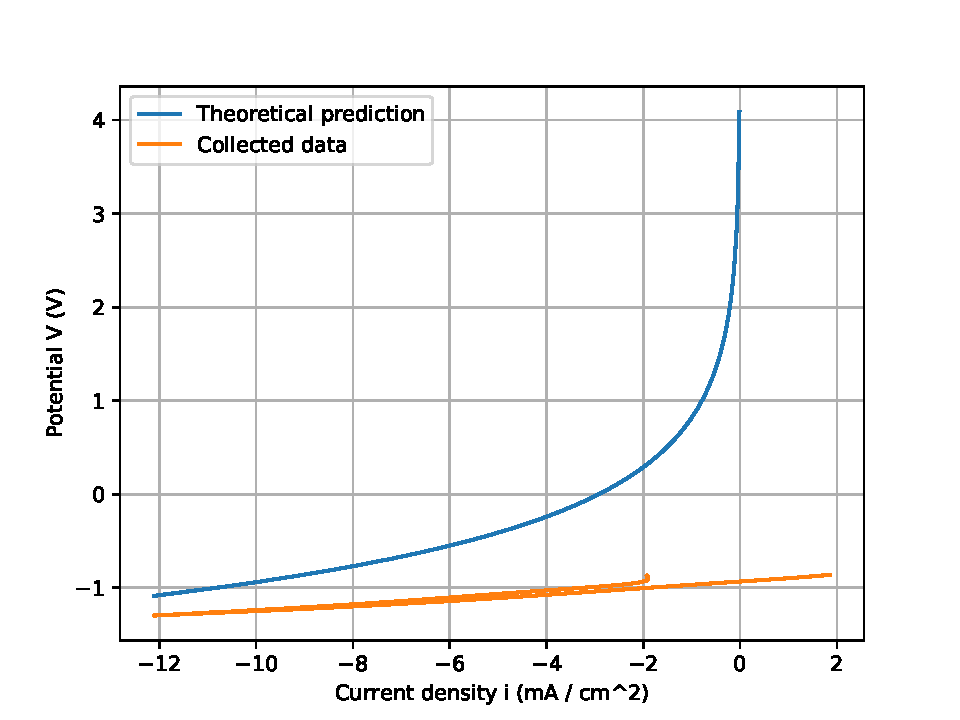
\includegraphics[width=\linewidth]{/home/sixten/water_electrolysis/data_analysis/plots/fin.pdf}
	\caption{Theoretical prediction using Tafel equation\ref{eq: tafel} versus collected data. Collected
	from \textbf{HER}.\newline \textbf{WE}: Pt, \textbf{CE}: Pt.\label{fig: tafel}}
\end{figure}
\section{Conclusion}
Using an experimental setup to generate data for different catalysts and consequently analyzed that data.
The best catalyst pair to maximise hydrogen production is found. 
\par
The overpotential is calculated \ref{eq: tafel} which unlocks the ability to compare the overpotential as a 
function of the current density then compare that theoretical prediction to the data that was gathered.
\ref{fig: tafel}. 
In an attempt to verify the predictions, tubes are set-up in order to collect the gas produced from
the reactions but, ultimately fail and the results are found to be inconclusive.
\pagebreak
\bibliography{bibliography}
\end{document}
